\documentclass[a4paper]{article}
\title{A Quick Introduction to TMM}
\author{Tatsuro Tanioka}
\date{\today}
% Recommended to compile with XeLaTeX

\usepackage[margin=1in]{geometry}
\usepackage{xcolor}
\usepackage{listings}
\lstdefinestyle{DOS}
{
    backgroundcolor=\color{black},
    basicstyle=\scriptsize\color{white}\ttfamily
}
\usepackage{natbib}
\usepackage{bibentry}
\nobibliography*
\usepackage{mathtools,amsthm}    % some advanced mathematics notation
%\usepackage{graphicx}            % easy inclusion and manipulation of images
\usepackage[draft]{graphicx}            % for draft- not displaying figures
\graphicspath{ {./Figures_tutorial/} }
\usepackage[font=small,labelfont=bf]{caption}
\usepackage{float}
\usepackage{microtype}           % just for fun: really hone in with the typography
\usepackage{booktabs}            % nice looking tables that present the content first and foremost
\usepackage{multicol}            % multiple columns in a local context
\usepackage[hidelinks]{hyperref} % clickable references in the output, but hide them visually
\usepackage{amssymb}
\usepackage{amsmath}
\usepackage[version=3]{mhchem}
\usepackage{newtxtext,newtxmath}
\usepackage{hyperref}
\usepackage{longtable}
\hypersetup{
    colorlinks=true,
    linkcolor=blue,
    filecolor=magenta,      
    urlcolor=cyan,
    citecolor=black,
%    pdftitle={Sharelatex Example},
%    bookmarks=true,
%    pdfpagemode=FullScreen,
    }
    
\urlstyle{same}

\def\noin{\noindent }
\def\CO{$\mathrm{CO_{2}}$ }
%%%%%%%%%%%%%----------------------------------------------------------
\begin{document}
\maketitle

\begin{abstract}
This document goes through how to use the Transport Matrix Model (TMM) using computational resources at the University of Minnesota's Minnesota Supercomputing Institution (MSI). All the source codes and documents (including this tutorial) that Tanioka made to TMM is available at my github website \url{(https://github.com/tanio003/tmm/tree/TT_Release)}.
\end{abstract}

\tableofcontents

\section{Setting up}

\subsection{Flow Chart}
Before you do anything, read ``README.txt'' by Samar Khatiwala at the following website: \\ \url{https://github.com/samarkhatiwala/tmm}. I will go over each of these steps specifically aimed at audiences using the computational cluster \emph{Mesabi}.
\begin{enumerate}
\item Installing and configuring PETSc
\item Downloading all the scripts and transport matrices into your own local directory
\item Compiling the model (we use the BGC model \verb/MOPS2/ for this example)
\item Running the model
\item Processing the model outputs
\item Displaying the model outputs
\end{enumerate}

\subsection{Steps}

\subsubsection{Step 0: Logging into MSI and Mesabi}
\noin Open the terminal (assuming that you have a MAC or Linux environment) on your computer and log in to MSI with your x500 account:
\begin{lstlisting}[style=DOS]
 $ ssh -Yt youremail@umn.edu
\end{lstlisting}

\noin Log in to Mesabi: 
\begin{lstlisting}[style=DOS]
 $ ssh -X mesabi
\end{lstlisting}

\noin Make a new directory called TMM2 in your home directory and enter into this directory. Everything related to TMM will go into this directory.
\begin{lstlisting}[style=DOS]
 $ mkdir TMM2
 $ cd TMM2
\end{lstlisting}

\subsubsection{Step 1: Installing and configuring PETSc}

\noin Download the latest version of PETSc and save it in your TMM2 directory and unzip this package. If opened properly, you should see the new directory petsc-3.13.5. 
\begin{lstlisting}[style=DOS]
 $ wget http://ftp.mcs.anl.gov/pub/petsc/release-snapshots/petsc-lite-3.13.5.tar.gz
 $ tar -xvf petsc-lite-3.13.5.tar.gz
 $ ls
 petsc-3.13.5
\end{lstlisting}

\noin Import the required modules: (1) impi, (2) impi/intel, and (3) cmake. Also make sure that you are using python 3, not python 2 (= default for MSI). 
\begin{lstlisting}[style=DOS]
 $ module purge 
 $ module load intel
 $ module load impi/intel
 $ module load cmake
 $ module load python3
 $ module list
Currently Loaded Modulefiles:
 1) intel/2018.release(default)   4) cmake/3.10.2(default)
 2) intel/2018/release            5) python3/3.7.1_anaconda
 3) impi/intel(default)
\end{lstlisting}

\noin Set up \verb/$PETSC_DIR/ to your petsc-3.13.5 directory. For your future uses, I would advise you to set \verb|$PETSC_DIR| in your \verb|.bashrc| as well. 
\begin{lstlisting}[style=DOS]
 $ export PETSC_DIR=$HOME/TMM2/petsc-3.13.5
 $ echo $PETSC_DIR 
 /.../TMM2/petsc-3.13.5
\end{lstlisting}

\noin Configure PETSc. Although this part is quite tricky you can copy and use my config file \\ ``\verb/reconfigure-arch-linux-c-opt.py/''. If the config file does not work properly, let me know and I can show you a way to compile without using this .py file. 
\begin{lstlisting}[style=DOS]
 $ cd petsc-3.13.5
 $ cp ~/../tanio003/TMM2/petsc-3.13.5/config/reconfigure-arch-linux-c-opt.py config/
 $ config/reconfigure-arch-linux-c-opt.py
\end{lstlisting}

\noin Don't worry about some warning signs. It takes few minutes to compile. If it's compiled properly you should see the notice ``Conifgure stage complete.'' Then build PETSc library:
\begin{lstlisting}[style=DOS]
 $ make all
\end{lstlisting}
Building process takes about 15-30 minutes. If you're very lucky it will go through in a single shot. But in most cases, it fails during the middle of the process. Don't worry if it fails the first time. Simply type ``\verb/$ make all/'' again and hopefully it will finish building from where it left off. If built properly, you should see the message ``Now to check if the libraries are working do:...''. Then type,
\begin{lstlisting}[style=DOS]
 $ make check
 ...
Completed test examples
\end{lstlisting}
If you get this far, you've managed to build the PETSc successfully and you're ready to go to the next step. If it failed, read the error messages, debug, and try again. \textbf{Building PETSc is harder than it looks} so you need to be patient. 

As more of a technical note, the procedure above uses the Intel compilers and Intel MPI library. By loading the cmake, the PETSc build system can learn more about the host machine. In addition to taking advantage of compiler optimizations and vectorization, the procedure above builds PETSc against the Intel Math Kernel Library (MKL) for BLAS, LAPACK and ScaLAPACK which gives a performance gain over the reference implementations. For the FORTRAN compiler, we specifically need to use \verb/mpiifort/, and not \verb/mpif90/ (the default compiler), because TMM codes are written in both F77 and F90. Also, since we don't require C++ for TMM we put the flag in the config file, \verb/--with-cxx=0/. The reason we need to use MPI compilers, not regular gcc compilers, is because we want to run PETSc in a parallel mode (i.e., by using the command \verb/mpiexec/ in the runscript). For more details about building PETSc please check out \url{https://www.mcs.anl.gov/petsc/documentation/installation.html}. 

\subsubsection{Step 2: Downloading all the scripts and transport matrices}
\begin{enumerate}
\item First download Matlab scripts from \\ 
\url{http://kelvin.earth.ox.ac.uk/spk/Research/TMM/tmm_matlab_code.tar.gz} and put into the first level of your TMM2 folder Path. You could also get my copy.
\begin{lstlisting}[style=DOS]
 $ cp -r ~/../tanio003/TMM2/tmm_matlab_code $HOME/TMM2/
\end{lstlisting}
\item Download transport matrices and related data for the model of your choice: \\ \url{http://kelvin.earth.ox.ac.uk/spk/Research/TMM/TransportMatrixConfigs/} and put into he first level of your TMM2 folder Path. You can download all 6 configurations but I warn you that \verb|MITgcm_ECCO_v4| and \verb|UVicKielIncrIsopycDiffTransient| take a very long time. For the ones that I have you could also grab my copy (e.g., to copy \verb|MITgcm_ECCO|):
\begin{lstlisting}[style=DOS]
 $ cp -r ~/../tanio003/TMM2/MITgcm_ECCO $HOME/TMM2/
\end{lstlisting}

\noin Alternatively, you can get download these TMM files from the web directly (e.g., to download \verb|MITgcm_ECCO|):
\begin{lstlisting}[style=DOS]
 $ wget kelvin.earth.ox.ac.uk/spk/Research/TMM/TransportMatrixConfigs/MITgcm_ECCO.tar
 $ tar -xvf MITgcm_ECCO.tar
\end{lstlisting}

\item Download miscellaneous data called OceanCarbon from \\ 
\url{http://kelvin.earth.ox.ac.uk/spk/Research/TMM/MiscData/}. You can get my copy by:
\begin{lstlisting}[style=DOS]
 $ cp -r ~/../tanio003/TMM2/OceanCarbon $HOME/TMM2/
\end{lstlisting}
\item Download source codes for TMM and models:
\begin{lstlisting}[style=DOS]
 $ git clone https://github.com/tanio003/tmm
\end{lstlisting}
 This directory (\verb|/TMM2/tmm|) contains the source codes from Khatiwala's master branch (``\verb|master|'') and my public release branch (``\verb|TT_Release|''). For our exercise, we will be using some of my new codes so you need to switch from the master branch to my branch in the newly created tmm directory:
\begin{lstlisting}[style=DOS]
 $ cd tmm
 (master) $ ls
 driver  HOWTO.txt  LICENSE.txt  models  README.txt
 (master) $ git checkout TT_Release
 (TT_Release) $ ls
 driver  HOWTO.txt  LICENSE.txt  models  README.txt  Tutorial_MSI
\end{lstlisting}
Notice that in the branch \verb|TT_Release|, there is a new directory \verb|Tutorial_MSI|, which was not present in the master branch. 

(Optional) If you want to make start making your own changes to the source codes, I would suggest making a new branch in your local computer (e.g.., \verb|yournewrepo|), and leave \verb|master| and \verb|TT_Release| untouched.
\begin{lstlisting}[style=DOS]
 (TT_Release) $ git checkout -b yournewrepo
 (yournewrepo) $ git branch --show-current
 yournewrepo
\end{lstlisting}
\item Set the environment variable TMMROOT to point to the top level of the TMM directory.
\begin{lstlisting}[style=DOS]
 (TT_Release) $ export TMMROOT=$HOME/TMM2/tmm
 (TT_Release) $ echo $TMMROOT
 /home/.../TMM2/tmm
\end{lstlisting}

For your future convenience, I would advise you to set \verb|$TMMROOT| in your \verb|.bashrc| as well so you don't need to set the variable every time you log in to MSI. 

\item To synchronize your \verb|tmm| folder with the remote repository (e.g., syncing \verb|TT_Release| with my updates), use the git pull command your terminal. I suggest you do this regularly to keep your files up to date.
\begin{lstlisting}[style=DOS]
 $ cd $TMMROOT
 $ git checkout TT_Release
 $ git pull origin TT_Release
\end{lstlisting}

\end{enumerate}

\subsubsection{Step 3: Compiling the model}
\noin Here, let's try compiling the biogeochemical MOPS. If you want to learn about the basic architecture of MOPS, read the model description paper by \citet{Kriest15} at \url{https://gmd.copernicus.org/articles/8/2929/2015/}. 

\begin{enumerate}
\item For each model there are model-specific source codes \\ (\verb|$TMMROOT/models/current/mops2/src/|); Matlab scripts \\ (\verb|$TMMROOT/models/current/mops2/matlab/|) to generate input data and read model output; and run scripts and other runtime data such as namelists in \\ 
\verb|$TMMROOT/models/current/mops2/runscripts/|. 

First, we create a new run directory. I make a new base directory called ``\verb|Runs|'' and in that directory, I make subdirectories for specific experiments. I call it \verb|Runs/MOPS/Test_spinup| and copy here all the files needed.

\begin{lstlisting}[style=DOS]
 $ cd ~/TMM2
 $ mkdir -p Runs/MOPS/TMM_spinup
 $ cd Runs/MOPS/TMM_spinup
 $ cp -p $TMMROOT/models/current/mops2.0/src/Makefile .
 $ cp -p -R $TMMROOT/models/current/mops2.0/matlab/* .
 $ cp -p $TMMROOT/models/current/mops2.0/runscripts/* .
\end{lstlisting}

\item Compile mops. Make sure that all the modules are loaded and \verb|$PETSC_DIR| is set correctly before you compile mops.
\begin{lstlisting}[style=DOS]
 $ module load intel
 $ module load impi/intel
 $ module load cmake
 $ make clean all
 $ make mops
\end{lstlisting}

\noin If compiled properly, you'd find a new executable ``mops'' created along with a bunch of objective .o files. 
\lstset{emph={mops,runscript_msi,Makefile}, emphstyle=\color{green}}
\begin{lstlisting}[style=DOS]
 $ ls
 BGC_INI.o                           n7fluxes28.m
 BGC_MODEL.o                         n7physics.m
 CAR_CHEM.o                          n7tracers28.m
 CAR_INI.o                           n7tracersavg28.m
 external_forcing_mops_biogeochem.o  perry1996-runoff-noarctic_noname.txt
 insolation.o                        perry1996-runoff_noname.txt
 load_output.m                       petsc_matvec_utils.o
 load_output_time_avg.m              petsc_signal_utils.o
 load_pco2.m                         process_output.m
 Makefile                            runscript
 make_input_files_for_mops_model.m   runscript_msi
 make_rivers.m                       tmm_external_bc.o
 misfit_mops_biogeochem.o            tmm_forcing_utils.o
 mops                                tmm_forward_step.o
 mops_biogeochem_copy_data.o         tmm_main.o
 mops_biogeochem_diagnostics.o       tmm_monitor.o
 mops_biogeochem_ini.o               tmm_profile_utils.o
 mops_biogeochem_misfit.o            tmm_timer.o
 mops_biogeochem_model.o             tmm_write.o
 mops_biogeochem_set_params.o
\end{lstlisting}
\lstset{emph={}, emphstyle=\color{green}}

\item Edit the file \ \verb/make_input_files_for_mops_model.m/. First thing to do is to make sure that variable \verb/base_path/ point to the right directory for the TMM configuration.
\lstset{language=matlab} 
\begin{lstlisting}[frame=single,basicstyle=\scriptsize,commentstyle=\color{blue}]
 % make_input_files_for_mops_model.m
 
 % Set toplevel path to GCMs configuration
 % base_path='/data2/spk/TransportMatrixConfigs/MITgcm_2.8deg';
 % base_path='/data2/spk/TransportMatrixConfigs/MITgcm_ECCO';
 % base_path='/data2/spk/TransportMatrixConfigs/MITgcm_ECCO_v4';
 base_path='~/TMM2/MITgcm_2.8deg';
 
 addpath(genpath('~/TMM2/tmm_matlab_code'));% add tmm_matlab_code to the search path
 oceanCarbonBasePath='~/TMM2/OceanCarbon';  % add OceanCarbon to the search path
 atmosDataPath=fullfile(oceanCarbonBasePath,'AtmosphericCarbonData');
\end{lstlisting}
\noin In the same matlab file, there are different switches (0 = no and 1 = yes). For this spin-up exercise, we \textbf{couple MOPS to a simple OCMIP-like carbon model} and \textbf{fix atmospheric $\mathrm{pCO_{2}}$ at 280 ppm}. So set the switches as following:
\begin{lstlisting}[frame=single,basicstyle=\scriptsize,commentstyle=\color{blue}]
 % make_input_files_for_mops_model.m
 ...
 periodicForcing=1 
 periodicMatrix=1
 
 dt=43200; % time step to use (43200s for ECCO and MIT2.8; 28800s for any other TMMs)
 
 rearrangeProfiles=1
 bigMat=0
 writeFiles=1
 writeTMs=1
 useCoarseGrainedMatrix=0
 writePCFiles=0
 
 READ_SWRAD=0                    % Read short-wave radiation?
 useCarbon=1                     % Use simple inorganic carbon model?
 useAtmModel=0                   % Use prognostic 1-box atmosphere?
 pCO2atm_ini=280.0               % Initial pco2?
 useTimeVaryingPrescribedCO2=0   % Use prescribed pco2 pathway?
 useVirtualFlux=1                % Use DIC and Alk to calculate E-P?
 empScaleFactor=1.0              % Scaling factor for E-P (default = 1)
 %-----------------------------------
 % Modified by Tatsuro Tanioka 200907 to allow for Atmospheric CO2 option
 % For a prescribed pCO2 run, useTimeVaryingPrescribedCO2=1 and choose a scenario
 
 % Available options: 'historical', 'RCP3PD', 'RCP45', 'RCP6' and 'RCP85'
 co2Scenario='RCP85';
 %-----------------------------------
\end{lstlisting}
\noin Then open MATLAB and run \verb/make_input_files_for_mops_model.m/
\begin{lstlisting}[style=DOS]
 $ module load matlab
 $ matlab -nodesktop
                                    < M A T L A B (R) >
                          Copyright 1984-2019 The MathWorks, Inc.
                     R2019a Update 5 (9.6.0.1174912) 64-bit (glnxa64)
                                      July 31, 2019
To get started, type doc.
For product information, visit www.mathworks.com.

>> make_input_files_for_mops_model
\end{lstlisting}
\noin This creates a bunch of periodic forcing files (\verb|xxx_01, xxx_02,...|), initial tracer concentrations \\ (\verb|po4ini.petsc, no3ini.petsc,...|), and binary files (.bin and .petsc) related to model geometry and forcing.
\end{enumerate}

\subsubsection{Step 4: Running the model}
\noin MSI systems use job queues to efficiently and fairly manage when computations are executed. The queuing system at MSI is called PBS (Portable Batch System) and to submit a job to a PBS queue users create PBS job scripts. PBS script contains information on the resources requested for calculation, as well as the commands for executing the calculation. 

Below is the custom PBS script for submitting a new job to run MOPS2 using Mesabi. It's called \verb|runscript_msi| and should be in the current directory already. Here is the first 11 lines:

\lstset{language=sh} 
\begin{lstlisting}[frame=single,basicstyle=\scriptsize]
 1  #!/bin/bash -l
 2  #PBS -l walltime=06:00:00,nodes=1:ppn=24,pmem=2580mb
 3  #PBS -m abe
 4  #PBS -j oe
 5  #PBS -M tatsurobkkuk@gmail.com
 6
 7  cd $PBS_O_WORKDIR
 8
 9  module load intel
 10 module load impi/intel
 11 module load cmake
 \end{lstlisting}

\noin The first line defines which type of shell the script will be read. Here we will use the \verb|bash|. The second line contains the PBS resource request. The current job will require about 6 hours, 1 node each with 24 processor cores (ppn), and 2580 megabytes of memory per core (pmem). 

The two lines containing \verb|#PBS -m abe|, and \verb|#PBS -M tatsurobkkuk@gmail.com|. are both commands having to do with sending message emails to the user.  The first of these lines instructs the PBS system to send a message email when the job aborts, begins, or ends. The second command specifies the email address to be used.  Using the message emails is recommended because the reason for a job failure can often be determined using information in the emails. The seventh line sets the directory at which commands are executed and the lines 8-11 loads the necessary software modules. 

The follwing lines (14$\sim$) contain the commands to execute and start a specific program. Different flags need to be change accordingly depending on the nature of experiments. For more information on different options available, read ``HOWTO.txt'' by S. Khatiwala located in \verb|$TMMROOT|. 
\begin{lstlisting}[frame=single,basicstyle=\scriptsize,commentstyle=\color{blue}]
 # 360 days per year with a time step of 2 steps per day:
 14 mpiexec -np 24 -hostfile $PBS_NODEFILE ./mops \   # number of cores, models
 15   -numtracers 9 \   # number of tracers (i.e. state variables)
 16   -i po4ini.petsc,dopini.petsc,oxyini.petsc,phyini.petsc,zooini.petsc,detini.petsc,
 no3ini.petsc,dicini.petsc,alkini.petsc \ # files for initialization of BGC state variables
 17   -me Ae \   # the name of the explicit transport matrix
 18   -mi Ai \   # the name of the implicit transport matrix
 19   -t0 0.0 -iter0 0 \ # starting time[years] starting time[timesteps]: for initial run
 20   -deltat_clock 0.0013888888888889 \  # ocean timestep length[years]: 2 timesteps/day
 21   -max_steps 2160000 \   # total number of timesteps to be evaluated (here 3000 yrs)
 22   -write_time_steps 72000 \ # output frequency(in timesteps, here every 100 yrs)
 23   -o po4out.petsc,dopout.petsc,oxyout.petsc,phyout.petsc,zooout.petsc,detout.petsc,
 no3out.petsc,dicout.petsc,alkout.petsc \ # files for output of 9 BGC state variables
 24   -external_forcing \ # calculate BGC explicitly
 25   -use_profiles \
 26   -nzeuph 2 \   # number of layers in euphotic zone (2 for MIT2.8, 6 for ECCO)
 27   -biogeochem_deltat 43200.0 -days_per_year 360.0 \ # ocean timestep[seconds]
 28   -burial_sum_steps 720 \   # sum burial over a period of 720 timesteps = 1 yr
 29   -pco2atm 280.0 \   # use fixed pCO2 of 280 ppm
 30   -use_virtual_flux \ # use the global surface mean DIC and Alk to calculate E-P
 31   -periodic_matrix \  # use of periodic transport matrix
 32   -matrix_cycle_period 1.0 -matrix_num_per_period 12 \ # the unit of time is year and 
 # circulation has a periodicity of 1 year; monthly mean tranport matrix (12 TMs/year)
 33   -periodic_biogeochem_forcing \  # periodic biogeochemical forcing
 34   -periodic_biogeochem_cycle_period 1.0 -periodic_biogeochem_num_per_period 12 \
 35   -num_biogeochem_steps_per_ocean_step 8 \ # the number of BGC timestep per ocean step
 36   -separate_biogeochem_time_stepping \  # timestep BGC model separately from ocean step
 37   -time_avg -avg_start_time_step 2159281 -avg_time_steps 60 \ 
 # initial timestep for avg concentrations (for final year); avg over 60 timestep = 1 month
 38   -avg_files po4avg.petsc,dopavg.petsc,oxyavg.petsc,phyavg.petsc,zooavg.petsc,
 detavg.petsc,no3avg.petsc,dicavg.petsc,alkavg.petsc \   # avg file names
 39   -calc_diagnostics -diag_start_time_step 2159281 -diag_time_steps 60 \
 # initial timestep for diagnostic fluxes (for final year); avg over 60 timesteps = 1 month
 40   -diag_files fbgc1.petsc,fbgc2.petsc,fbgc3.petsc,fbgc4.petsc,fbgc5.petsc,fbgc6.petsc,
 fbgc7.petsc \ # diagnsotic flux files names
 41     > log   # outputting to logfile
\end{lstlisting}

\noin Currently BGC model writes the following 7 diagnostics into the different files:
\begin{enumerate}
\item \verb|fbgc1.petsc|: primary production in each box [mmol P/m3/oceantimestep]
\item \verb|fbgc2.petsc|: zooplankton grazing in each box [mmol P/m3/oceantimestep]
\item \verb|fbgc3.petsc|: detritus sedimentation through upper boundary of \\ each box [mmol P/m2/oceantimestep]
\item \verb|fbgc4.petsc|: remineralization of detrius and DOP in each box [mmol P/m3/oceantimestep]
\item \verb|fbgc5.petsc|: river runoff [mmol P/m3/oceantimestep]
\item \verb|fbgc6.petsc|: nitrogen fixation [mmol N/m3/oceantimestep]
\item \verb|fbgc7.petsc|: denitrification [mmol P/m3/oceantimestep]
\end{enumerate}

\noin To submit the job to the queue, type on the command line:
\begin{lstlisting}[style=DOS]
 $ chmod u+x runscript_msi
 $ qsub runscript_msi
\end{lstlisting}

\noin To check your job status at MSI, type:
\begin{lstlisting}[style=DOS]
 $ showq -u yourusername
\end{lstlisting}

\subsubsection{Step 5: Processing the model outputs}

\noin When the run is completed, you should receive an email from MSI (if you set it so in the runscript). You should also check you log file and the bottom of the log file should say ``Wall clock time xxx seconds''. As the output files are binary and cannot be opened on its own, we have to convert from the binary format into either netcdf (.nc) or Matlab (.mat) files using Matlab scripts.

\vspace{5mm}
\noin (Option 1, recommmended): To convert to \textbf{.nc} files you are going to use the following 5 scripts:
\begin{enumerate}
\item \verb|n7tracers28.m|: This file converts each tracer snapshot .petsc file (e.g., po4put.petsc) into a single .nc file. The MATLAB syntax is:
\begin{lstlisting}[style=DOS]
 >> n7tracers28('filename1.nc')
\end{lstlisting}
Make sure to set the basepath correctly and useCarbon=1 (when carbon model is used) and make sure that there is no .nc file with the same name already in the directory.

\item\verb|n7tracersavg28.m|: This file converts each tracer time-averaged .petsc file (e.g., po4avg.petsc) into a single .nc file. The MATLAB syntax is:
\begin{lstlisting}[style=DOS]
 >> n7tracersavg28('filename2.nc')
\end{lstlisting}
Make sure to set the basepath correctly and useCarbon=1 (when carbon model is used) and make sure that there is no .nc file with the same name already in the directory.

\item\verb|n7fluxes28.m|: This file converts each diagnostic flux .petsc file (e.g., fbgc1.petsc) into a single .nc file. The MATLAB syntax is:
\begin{lstlisting}[style=DOS]
 >> n7fluxes28('filename3.nc')
\end{lstlisting}
Make sure to set the basepath correctly and make sure that there is no .nc file with the same name already in the directory.

\item\verb|n7physics.m|: This file makes single .c files with monthly mean temperature and salinity. The MATLAB syntax is:
\begin{lstlisting}[style=DOS]
 >> n7physics('filename4.nc')
\end{lstlisting}
Make sure to set the basepath correctly and make sure that there is no .nc file with the same name already in the directory.

\item\verb|load_pco2.m|: This file makes a global mean atmospheric $\mathrm{pCO_{2}}$ file (``pco2.nc'') and surface $\mathrm{CO_{2}}$ air-sea flux file (``co2airseaflux.nc''). $\mathrm{CO_{2}}$ is in ppm and $\mathrm{CO_{2}}$ air-sea flux is in [mmol C/m2/timestep] (positive flux means $\mathrm{CO_{2}}$ is going into the sea from air). The MATLAB syntax is 
\begin{lstlisting}[style=DOS]
 >> load_pco2
\end{lstlisting}
Make sure to set the basepath and the $\mathrm{CO_{2}}$ run options correctly.

\item\verb|process_output.m| (optinal): To run all 5 scripts at once, edit and use this file. The MATLAB syntax is 
\begin{lstlisting}[style=DOS]
 >> process_output
\end{lstlisting}

\end{enumerate}

\noin (Option 2): To convert to \textbf{.mat} files you are going to run 2 scripts:
\begin{enumerate}

\item \verb|load_output.m|: This file converts each tracer snapshot .petsc file (e.g., po4put.petsc) to .mat file. Make sure to edit the \verb|base_path| and add \verb|tmm_matlab_code| to search path in lines 2 and 3.
\item \verb|load_output_time_avg.m|: This file converts each tracer average concentration .petsc file (e.g., po4avg.petsc) to .mat file. Make sure to edit the \verb|base_path| and search path correctly.
\item Unfortunately I don't have scripts for creating .mat diagnostic flux files, physics files, and $\mathrm{CO_{2}}$ files. But this should not be too hard to do and all you have to do is to modify other .m files.

\end{enumerate}

\subsubsection{Step 6: Displaying the model outputs}
\noin (Option 1): To view .nc files, I recommend the software \emph{Ferret} developed by NOAA. It is already installed in MSI, and to launch Ferret, type on the command line:
\begin{lstlisting}[style=DOS]
 $ ls *.nc
 filename1.nc filename2.nc filename3.nc filename4.nc co2airseaflux.nc pco2.nc
 $ module load ferret
 $ ferret
 	NOAA/PMEL TMAP
 	FERRET v6.82
 	Linux 2.6.32-279.1.1.el6.x86_64 64-bit - 08/03/12
 	14-Sep-20 14:49

yes? load filename1.nc
yes? sho d
     currently SET data sets:
    1> ./filename1.nc  (default)
 name     title                             I         J         K         L
 PO4                                       1:128     1:64      1:15      1:31
 DOP                                       1:128     1:64      1:15      1:31
 OXYGEN                                    1:128     1:64      1:15      1:31
 PHYTO                                     1:128     1:64      1:15      1:31
 ZOO                                       1:128     1:64      1:15      1:31
 DET                                       1:128     1:64      1:15      1:31
 NO3                                       1:128     1:64      1:15      1:31
 DIC                                       1:128     1:64      1:15      1:31
 ALK                                       1:128     1:64      1:15      1:31
\end{lstlisting}
I won't go into too much detail here but to learn more about Ferret, visit NOAA's website and take a tutorial at \url{https://ferret.pmel.noaa.gov/Ferret/documentation/ferret-tutorials}. You can make all kinds of graphs and figures with Ferret.

\vspace{5mm}
\noin (Option 2): If you want to visualize .mat files, I recommend the MATLAB package \verb|m_map|. Again, I would not go into much detail here but if you want to learn about it, download the package and take the tutorial from the developer's website: \url{https://www.eoas.ubc.ca/~rich/map.html}. Compared to Ferret, you have more freedom for customizing graphs but the downside is that you are going to have to write much longer codes.

\section{Case Studies}
\subsection{Study 1: Postindustrial $\mathrm{CO_{2}}$ uptake with MOPS+MIT2.8}
\noin In the first case study, we will simulate postindustrial $\mathrm{CO_{2}}$ uptake using MOPS and MITgcm2.8 under IPCC's RCP8.5 scenario from 1765 to 2265. We are going to do the continuous run from the spinup run (Section 1) so make sure that you have completed that run before you proceed.
\begin{enumerate}

\item Update source codes in your \verb|tmm| directly by doing \verb|git pull| from the remote repository.
\begin{lstlisting}[style=DOS]
 $ cd $TMMROOT
 $ git checkout TT_Release
 $ git pull origin TT_Release
\end{lstlisting}

\item Make a new run directory. Let's call it \verb|Test_co2historyRCP85| and copy all the files needed into this directory.
\begin{lstlisting}[style=DOS]
 $ cd ~/TMM2
 $ mkdir -p Runs/MOPS/TMM_co2historyRCP85
 $ cd Runs/MOPS/TMM_co2historyRCP85
 $ cp -p $TMMROOT/models/current/mops2.0/src/Makefile .
 $ cp -p -R $TMMROOT/models/current/mops2.0/matlab/* .
 $ cp -p $TMMROOT/models/current/mops2.0/runscripts/* .
\end{lstlisting}

\item Compile mops as we have done in the spinup run. Don't forget to load modules and make sure that environmental variables \verb|$TMMROOT| and \verb|$PETSC_DIR| are set up properly.
\begin{lstlisting}[style=DOS]
 $ make clean all
 $ make mops
\end{lstlisting}

\item Copy the file \verb|pickup.petsc| from the spinup run directory into the current working directory. This petsc files contains the tracer concentrations from the final year of the run and is required for the continuous run.
\begin{lstlisting}[style=DOS]
 $ cp ../Test_spinup/pickup.petsc .
\end{lstlisting}

\noin Also, copy the file \verb|pickup_runoff.bin| from the spinup run directory. This binary file contains the global sedimentation from the final year of the previous run.
\begin{lstlisting}[style=DOS]
 $ cp ../Test_spinup/pickup_runoff.bin .
\end{lstlisting}

\item Edit the input generation file (\verb|make_input_files_for_mops_model.m|). The key here is to set \\ \verb|useTimeVaryingPrescribedCO2=1| and choosing the appropriate \verb|co2Scenario|, in this case RCP85. 
\lstset{language=matlab} 
\begin{lstlisting}[frame=single,basicstyle=\scriptsize,commentstyle=\color{blue}]
 % make_input_files_for_mops_model.m
 
 % Set toplevel path to GCMs configuration
 % base_path='/data2/spk/TransportMatrixConfigs/MITgcm_2.8deg';
 % base_path='/data2/spk/TransportMatrixConfigs/MITgcm_ECCO';
 % base_path='/data2/spk/TransportMatrixConfigs/MITgcm_ECCO_v4';
 base_path='~/TMM2/MITgcm_2.8deg';
 
 addpath(genpath('~/TMM2/tmm_matlab_code'));% add tmm_matlab_code to the search path
 oceanCarbonBasePath='~/TMM2/OceanCarbon';  % add OceanCarbon to the search path
 atmosDataPath=fullfile(oceanCarbonBasePath,'AtmosphericCarbonData');
 ...
  
 READ_SWRAD=0                    % Read short-wave radiation?
 useCarbon=1                     % Use simple inorganic carbon model?
 useAtmModel=0                   % Use prognostic 1-box atmosphere?
 pCO2atm_ini=280.0               % Initial pco2? (will be ignored as useAtmModel=0)
 useTimeVaryingPrescribedCO2=1   % Use prescribed pco2 pathway?
 useVirtualFlux=1                % Use DIC and Alk to calculate E-P?
 empScaleFactor=1.0              % Scaling factor for E-P (default = 1)
 %-----------------------------------
 % Modified by Tatsuro Tanioka 200907 to allow for Atmospheric CO2 option
 % For a prescribed pCO2 run, useTimeVaryingPrescribedCO2=1 and choose a scenario
 
 % Available options: 'historical', 'RCP3PD', 'RCP45', 'RCP6' and 'RCP85'
 co2Scenario='RCP85';
 %-----------------------------------
\end{lstlisting}

\item Open Matlab and make input files:
\begin{lstlisting}[style=DOS]
 $ matlab -nodesktop
 ...
 >> make_input_files_for_mops_model
\end{lstlisting}

\item Edit \verb|runscript_msi|. Important changes are commented with blue. You can manually edit the script or copy my script from \verb|~/../tanio003/TMM2/Runs/MOPS/Test_co2historyRCP85|.
\lstset{language=sh} 
\begin{lstlisting}[frame=single,basicstyle=\scriptsize,commentstyle=\color{blue}]
  1 #!/bin/bash -l
  2 #PBS -l walltime=01:00:00,nodes=1:ppn=24,pmem=2580mb
  3 #PBS -m abe
  4 #PBS -j oe
  5 #PBS -M tatsurobkkuk@gmail.com
  6
  7 cd $PBS_O_WORKDIRP
  8
  9 module load intel
 10 module load impi/intel
 11 module load cmake
 12
 13 # 360 days per year with a time step of 2 steps per day:
 14 mpiexec -np 24 -hostfile $PBS_NODEFILE ./mops \
 15   -numtracers 9 \
 16   -pickup pickup.petsc \   # read initial values from file
 17   -me Ae \
 18   -mi Ai \
 19   -t0 1765.0 -iter0 0 \   # start from year 1765
 20   -deltat_clock 0.0013888888888889 \   
 21   -max_steps 360000 \  # run for 720*500 timesteps = 500 years
 22   -write_time_steps 7200 \   # output every 720*10 timestep = 10 years
 23   -o po4out.petsc,dopout.petsc,oxyout.petsc,phyout.petsc,zooout.petsc,
 detout.petsc,no3out.petsc,dicout.petsc,alkout.petsc \
 24   -external_forcing \
 25   -use_profiles \
 26   -nzeuph 2 \
 27   -biogeochem_deltat 43200.0 -days_per_year 360.0 \
 28   -burial_sum_steps 720 \
 29   -runoff_ini_file pickup_runoff.bin \ # read global sedimentation of previous run
 30   -periodic_matrix \
 31   -pco2atm_history TpCO2.bin,pCO2atm.bin \ # read prescribed pCO2 and time
 32   -use_virtual_flux \
 33   -matrix_cycle_period 1.0 -matrix_num_per_period 12 \
 34   -periodic_biogeochem_forcing \
 35   -periodic_biogeochem_cycle_period 1.0 -periodic_biogeochem_num_per_period 12 \
 36   -num_biogeochem_steps_per_ocean_step 8 \
 37   -separate_biogeochem_time_stepping \
 38   -time_avg -avg_start_time_step 169201 -avg_time_steps 720 \ 
 # output annual avg. from year 2000 (235 years after 1765)
 39   -avg_files po4avg.petsc,dopavg.petsc,oxyavg.petsc,phyavg.petsc,zooavg.petsc,
 detavg.petsc,no3avg.petsc,dicavg.petsc,alkavg.petsc \
 40   -calc_diagnostics -diag_start_time_step 169201 -diag_time_steps 720 \ 
 # output annual mean fluxes from 2000 (235 years after 1765)
 41   -diag_files fbgc1.petsc,fbgc2.petsc,fbgc3.petsc,fbgc4.petsc,fbgc5.petsc,
 fbgc6.petsc,fbgc7.petsc \
 42   > log
\end{lstlisting}

\item Submit the job to MSI queue.
\begin{lstlisting}[style=DOS]
 $ qsub runscript_msi
\end{lstlisting}

\item Processing and outputting results. Use 5 Matlab scripts \\ (\verb|n7tracers28.m,n7tracersavg28.m,n7fluxes28.m,n7physics.m,load_pco2.m|) to create .nc files. Here, I will show you how to plot $\mathrm{CO_{2}}$ timeseries and global annual mean air-sea flux of $\mathrm{CO_{2}}$ using Ferret. The script is also at \verb|~/../tanio003/TMM2/Runs/MOPS/Test_co2historyRCP85/analyzeoutput.jnl|. 
\begin{lstlisting}[style=DOS]
 $ ferret
  	NOAA/PMEL TMAP
 	PyFerret v7.5 (optimized)
 	Linux 4.15.0-1071-azure - 03/31/20
 	16-Sep-20 14:49
 yes? use pco2.nc
 yes? use co2airseaflux.nc
 yes? set w 1;plot/d=1/hlimits=1800:2120/vlimits=200:1200/title="pCO2 RCP8.5" pco2
 yes? ppl XLAB Year
 yes? ppl YLAB pCO2 (ppm)
 yes? ppl PLOT
 yes? set w 2 ; sha/d=2/x=-180:180/lev=(-Inf)(-4,4,0.8)(Inf)/palette=cmocean_balance/
 title="Annual CO2 flux (mol C m-2 yr-1)" co2air_to_sea_flux[l=10]*2*360/1000*(-1);go fland
 yes? set w 3 ; sha/d=2/x=-180:180/lev=(-Inf)(-4,4,0.8)(Inf)/palette=cmocean_balance/
 title="Annual CO2 flux (mol C m-2 yr-1)" co2air_to_sea_flux[l=100]*2*360/1000*(-1);go fland
 yes? set w 4; plot/d=2/hlimits=2000:2100/vlimits=-7:0/
 title="Ocean-atmosphere CO2 flux (PgC yr-1)" co2air_to_sea_flux[x=@din,y=@din]*2*360/1000*12/1e15*(-1)
\end{lstlisting}
(Note: Here, I'm actually using the new version of the Ferret called PyFerret and some of the commands may not be compatible with the older version that is pre-installed at MSI. To install PyFerret in your MSI directory, see Appendix and follow instructions. Also, visit \url{https://github.com/NOAA-PMEL/PyFerret/} for more information. \emph{I highly recommend PyFerret.})

\begin{figure}[b!]   % Insert Figure 1 here
   \centering
   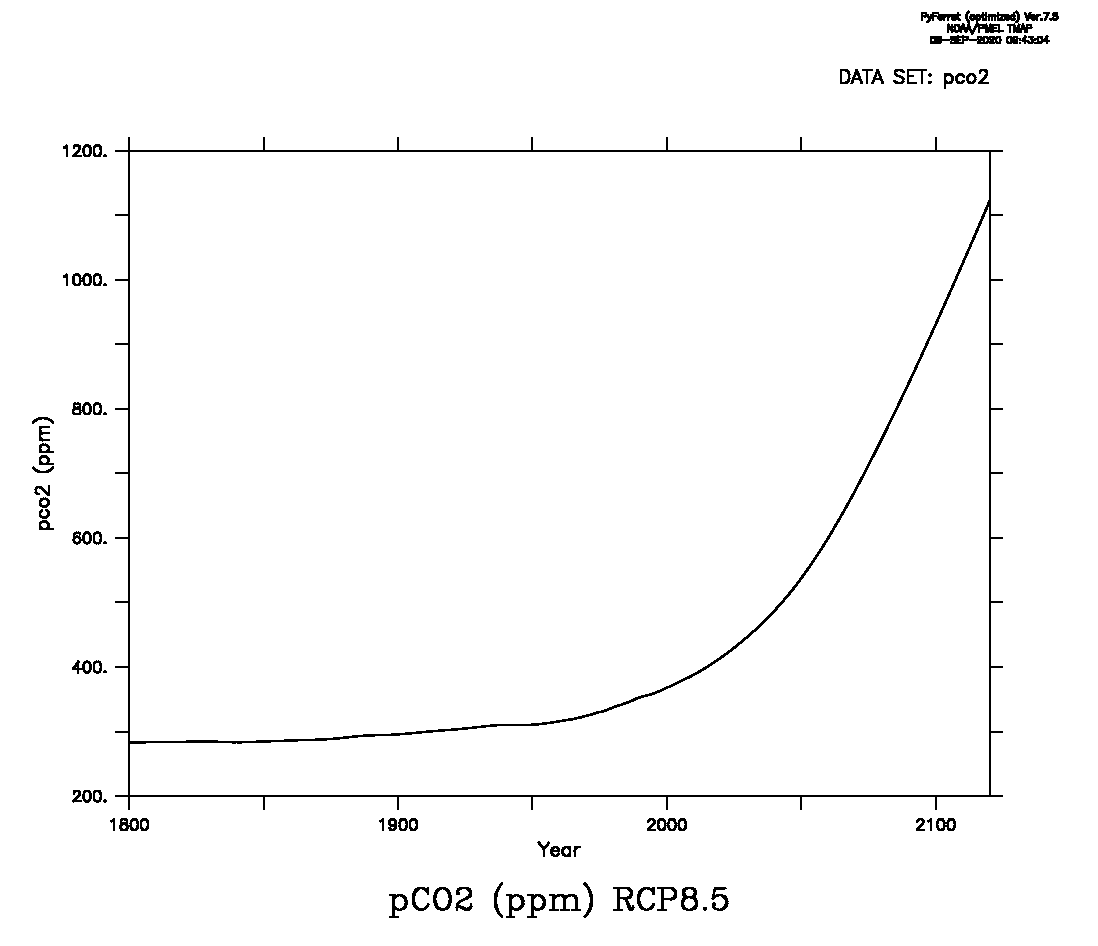
\includegraphics[width=10cm]{pco2RCP85.pdf}
   \caption[]{$\mathrm{CO_2}$ concentration pathway under RCP8.5 scenario \citep{Meinshausen11}.}
   \label{fig:pco2RCP85}
\end{figure}

Figure \ref{fig:pco2RCP85} (\emph{Ferret:w 1}) shows the change in $\mathrm{CO_2}$ under RCP8.5 scenario. There is a rapid increase in \CO concenctration from the late 1990s. 

Figure \ref{fig:airseamap} compares annual mean $\mathrm{CO_2}$ flux in 2010 (\emph{Ferret:w 2}) and 2100 (\emph{Ferret:w 3}). Notice that in 2010, large parts of the equatorial regions are net source of $\mathrm{CO_2}$ but in 2100, larger parts are becoming sink. Also, greater part of the Southern Ocean is also expected to absorb more  $\mathrm{CO_2}$ in 2100 compared to 2010. 

Figure \ref{fig:airseamapWoolf} is a $\mathrm{CO_2}$ flux in 2010 from a study by \cite{Woolf19} who used Surface $\mathrm{CO_2}$ atlas and wind data. If you compare with the left panel of Figure  \ref{fig:airseamap}, you can see that our MOPS model does a quite good job in reproducing the large scale pattern.

\begin{figure}[h!]   % Insert Figure 2 here
   \centering
   \begin{minipage}{0.45\columnwidth}
      \centering
      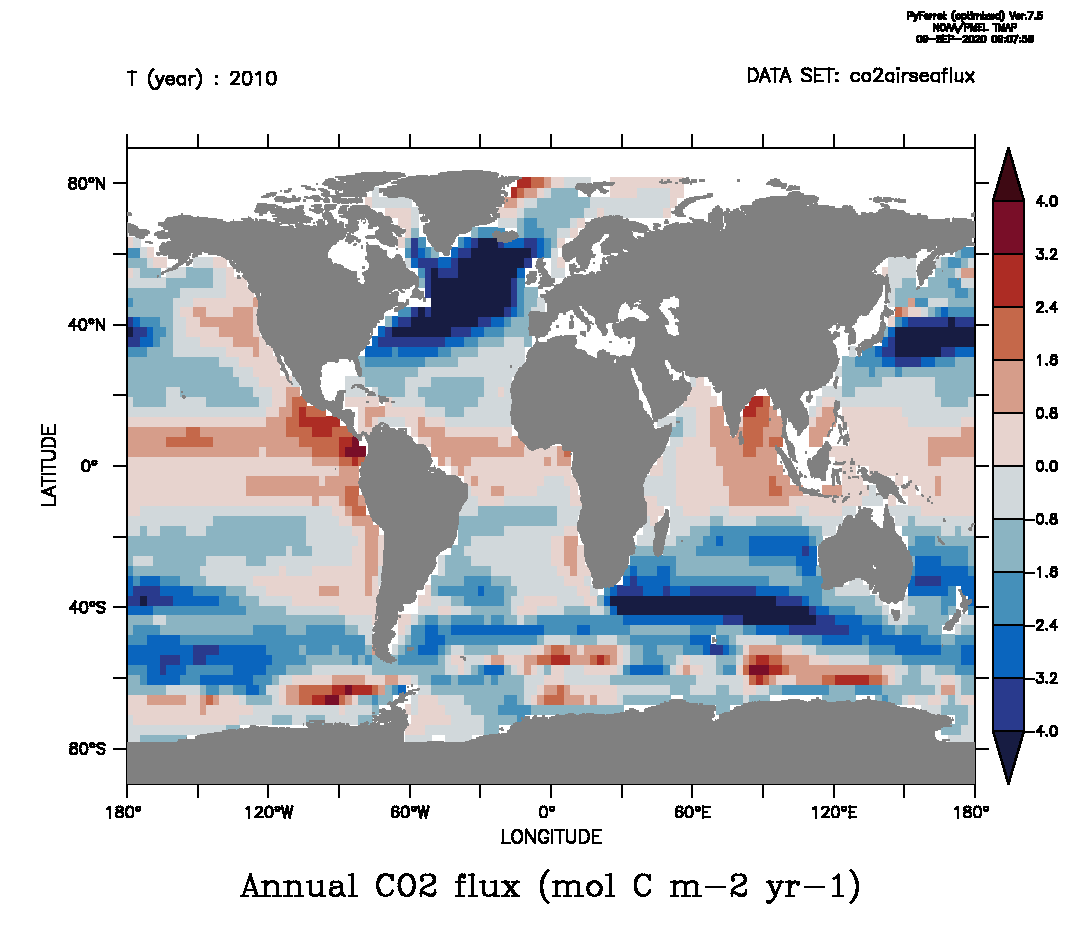
\includegraphics[width=\columnwidth]{airseaflux2010.pdf}
   \end{minipage}
   \begin{minipage}{0.45\columnwidth}
      \centering
      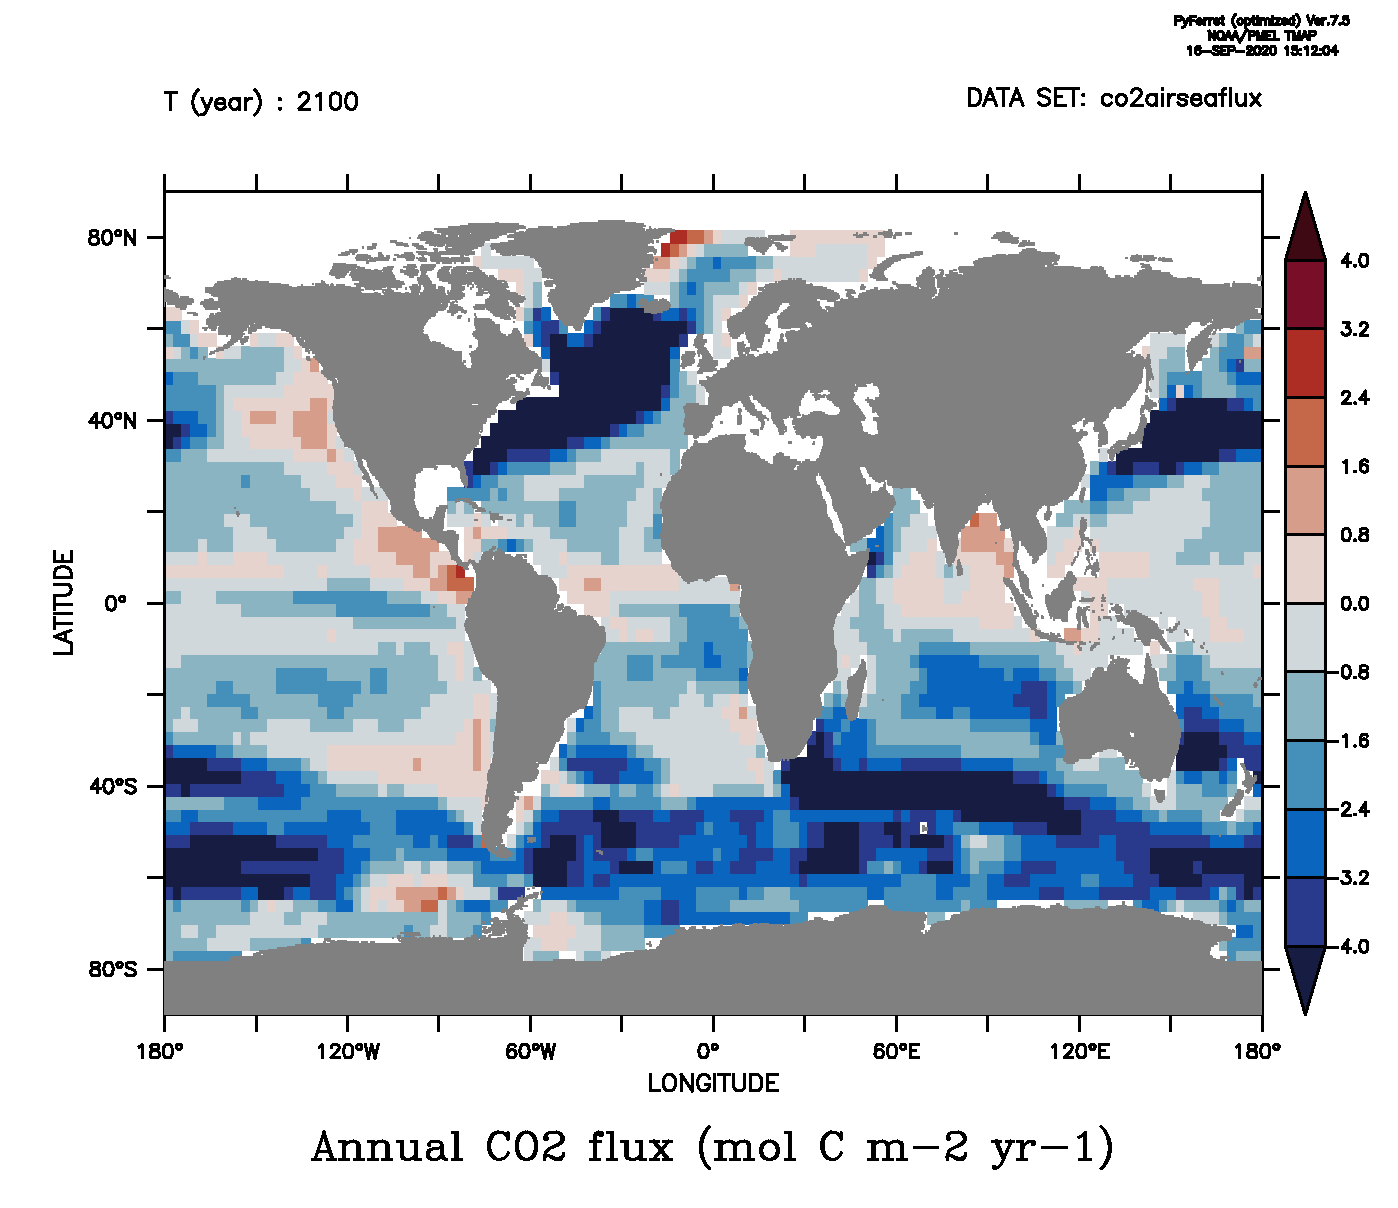
\includegraphics[width=\columnwidth]{airseaflux2100.pdf}
   \end{minipage}
   \caption[]{Modeled map of annual $\mathrm{CO_{2}}$ flux for 2010 (Left) and for 2100 (Right). Upward fluxes are defined as positive.}
   \label{fig:airseamap}
\end{figure}

\begin{figure}[h!]   % Insert Figure 3 here
   \centering
   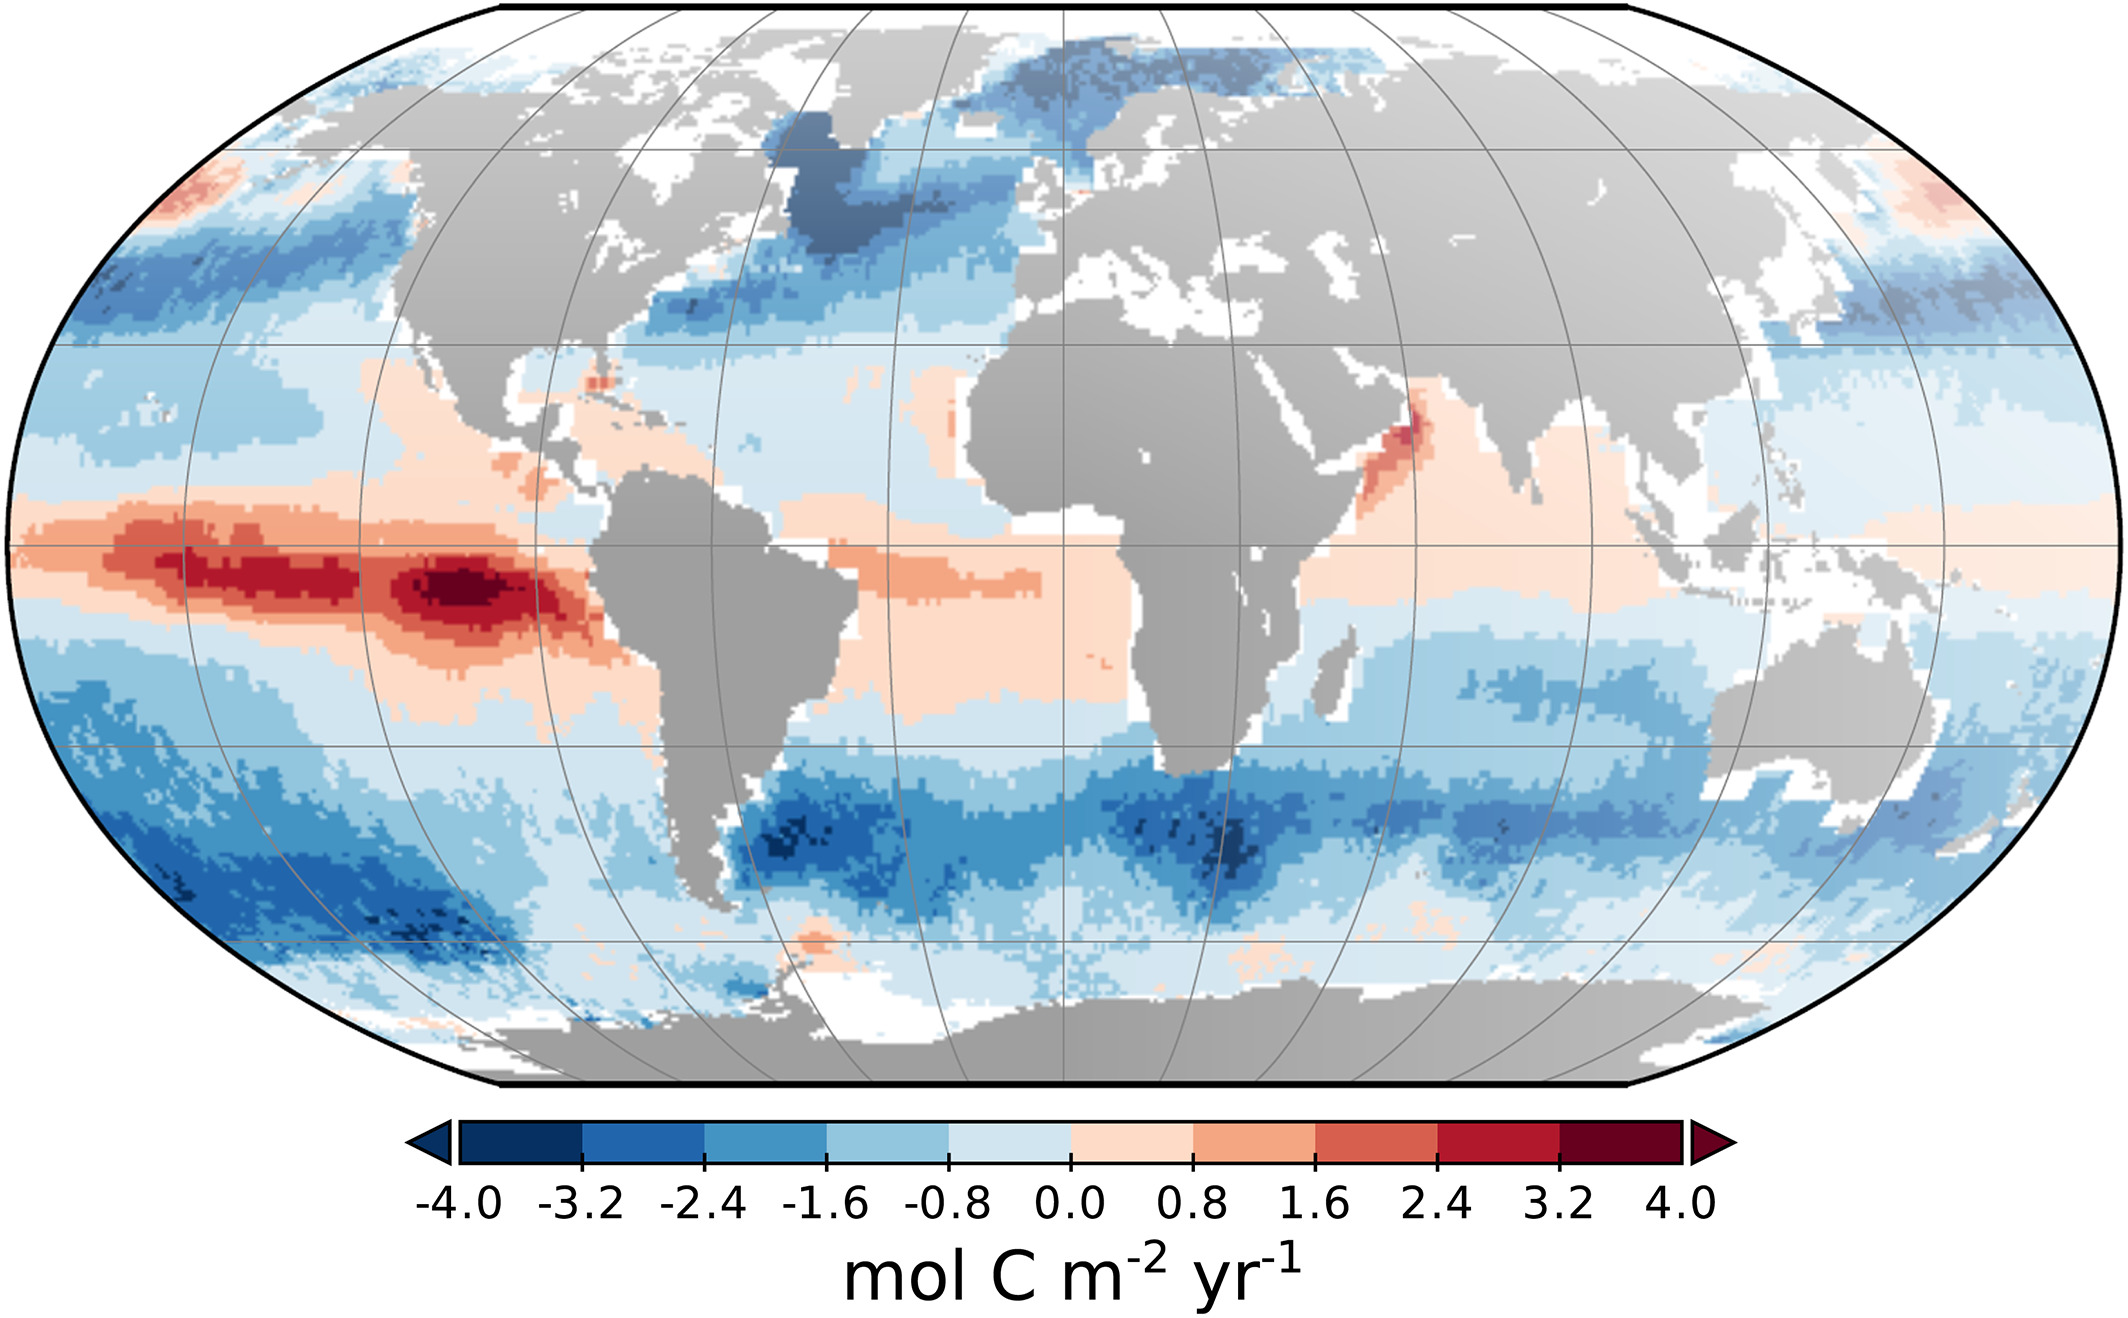
\includegraphics[scale=0.1]{Woolf19_GBC_Fig1.jpg}
   \caption[]{Map of annual $\mathrm{CO_{2}}$ flux in 2010 from $\mathrm{CO_2}$ and wind data \citep{Woolf19}. Compare this with Figure \ref{fig:airseamap}.}
   \label{fig:airseamapWoolf}
\end{figure}

Figure \ref{fig:airseatimeseries} (\emph{Ferret:w 4}) is a globally integrated sea-air $\mathrm{CO_2}$ flux projections under RCP8.5 scenario.The negative value means net uptake of $\mathrm{CO_2}$ by ocean. For a comparison, we show the similar projection using the CESM and CMIP5 (Figure \ref{fig:airseatimeseries_cmip5}a-b.) from \cite{Lovenduski16}. Again, notice that MOPS's result is largely consistent in terms of the magnitude. 

\begin{figure}[H]   % Insert Figure 4 here
   \centering
   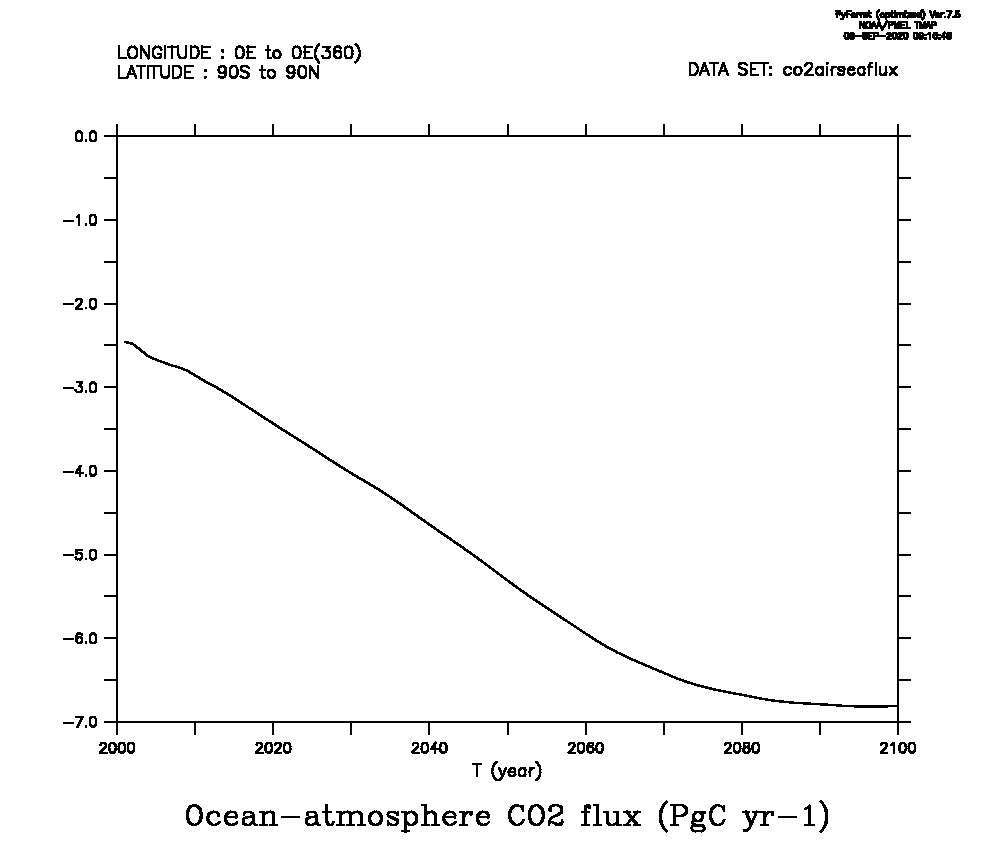
\includegraphics[scale=0.35]{airseaflux_timeseries2000to2100.pdf}
   \caption[]{Modeled annual-mean globally integrated sea-air $\mathrm{CO_2}$ flux projections under RCP8.5 scenario.}
   \label{fig:airseatimeseries}
\end{figure}

\begin{figure}[H]   % Insert Figure 5 here
   \centering
   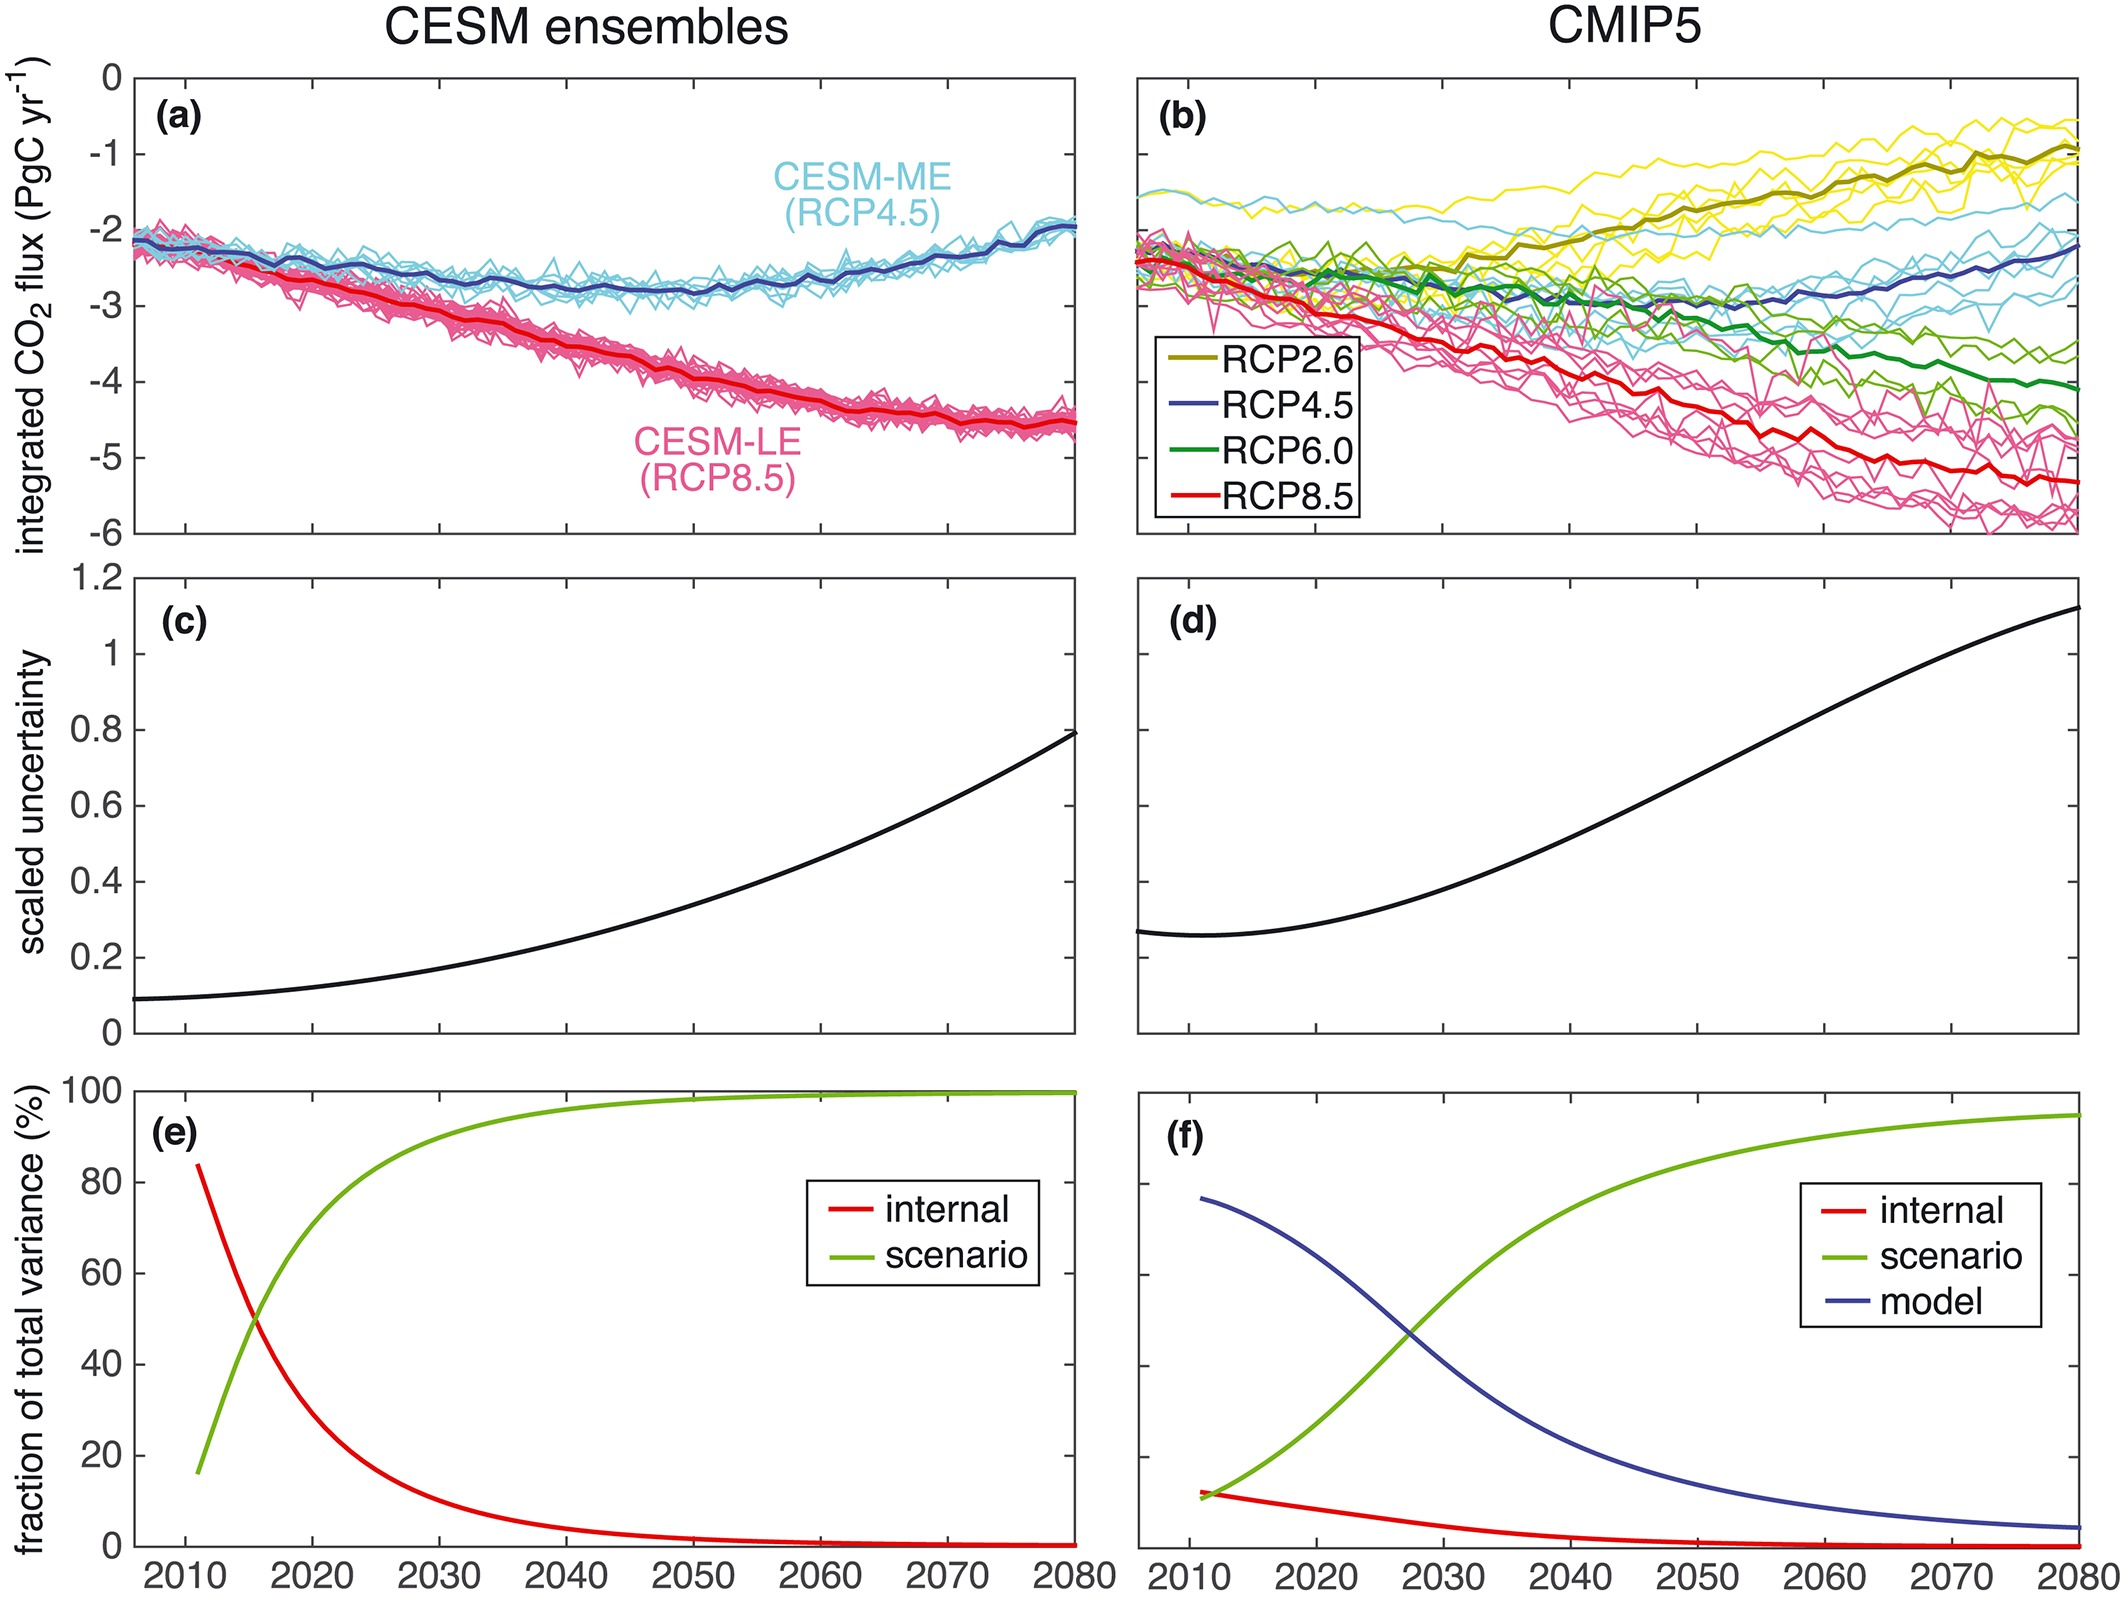
\includegraphics[trim=0 760 0 0,clip,scale=0.3]{Lovenduski16_GBC_Fig2.jpg}
   \caption[]{Modeled annual-mean globally integrated sea-air $\mathrm{CO_2}$ flux projections \citep{Lovenduski16} with CESM (a) and CMIP5 models (b). Compare this with Figure \ref{fig:airseatimeseries}.}
   \label{fig:airseatimeseries_cmip5}
\end{figure}

\end{enumerate}

\subsection{Study 2: Using MOBI+UVic to simulate isotope dynamics}

For this study, we will explore ocean biogeochemical dynamics using the second version of MOBI (Model of Ocean Biogeochemistry and Isotopes). MOBI includes:
\begin{itemize}
\item \ce{NO3}, \ce{PO4}, and DFe as interactive nutrients.
\item 3 Phytoplankton classes (diazotrophs, coccolithophores, and other phytoplankton).
\item Zooplankton.
\item Detritus (dead POM).
\item \ce{CaCO3} is a prognostic variable and its production is calculated as a fraction of the detrirus produced by coccolithophores and zooplankton and it is sinking into the deep ocean where it dissolves.
\item Nitrogen (\ce{^15N}) and carbon (\ce{^13C}) isotopes are included in all compartments.
\item Radiocarbon (\ce{^14C}) is included only in the DIC compartment.
\item Dissolved \ce{O2} controls the water column denitrification. Benthic denitrification is calculated considerting subgridscale bathymetry.
\item DOM is calculated separately for C, N, and P (DOC, DON, DOP).
\item The most complex configuration has a total of 30 prognostic tracers.
\end{itemize}
\noin To learn different configurations of MOBI, refer to the primer by A. Schmittner (\url{https://github.com/tanio003/tmm/blob/TT_Release/Tutorial_MSI/MOBI2.0_Schmittner.pdf}). 

\textbf{In our exercise, we will try conducting a spin-up run for 3000 yrs using 30 prognostic tracers. Instructions will mostly follow that of S. Khatiwala.}

\begin{enumerate}

\item Download the compatible versions of UVic ESCM 2.9 in the first level of your TMM directory
\begin{lstlisting}[style=DOS]
 $ cd ~/TMM2
 $ git clone https://github.com/your_github_username/UVic2.9
\end{lstlisting}

\item Download the TMM called \verb|UVicOSUpicdefault|. Although you can download the original TMM from the Samar's repository, I found out when I did the preliminary test that the original TMM does not have the flow field for river discharge. Therefore, I had to import the ``foreign'' river discharge field from another TMM called  \verb|UVicKielIncrIsopycDiff| (\emph{Maybe we could contact Samar to ask for the full configuration for} \verb|UVicOSUpicdefault| \emph{with river discharge?}). To copy my TMM, 
\begin{lstlisting}[style=DOS]
 $ cp -r ~/../tanio003/TMM2/UVicOSUpicdefault_with_discharge $HOME/TMM2/
\end{lstlisting}

\noin Currently, MOBI can only be coupled to this TMM configuration (\verb|UVicOSUpicdefault_with_discharge|) because other TMMs like MITgcm models do not have bathymetry profile and hydrothermal Fe input masks.

\item Make a Run directory for TMM-MOBI. For this run, I call it \verb|Runs/MOBI/Test_spinup|. Copy \\ \verb|mobi2.0/src/Makefile| and \verb|mobi2.0/src/MOBI_TMM_OPTIONS.h| to this directory. 
\begin{lstlisting}[style=DOS]
 $ cd ~/TMM2
 $ mkdir -p Runs/MOBI/TMM_spinup
 $ cd Runs/MOBI/TMM_spinup
 $ cp -p $TMMROOT/models/current/mobi2.0/src/Makefile .
 $ cp -p $TMMROOT/models/current/mobi2.0/src/MOBI_TMM_OPTIONS.h . 
\end{lstlisting}
\noin Also, following the instructions at the top of Makefile, set the environmenta variable \verb|$UVICESCMROOT| to point to the top level of the UVic ESCM 2.9. Add this to your \verb|.bashrc| for cd your future convenience.
\begin{lstlisting}[style=DOS]
 $ export UVICESCMROOT=$HOME/TMM2/UVic2.9
 echo $UVICESCMROOT
 /home/...//TMM2/UVic2.9
\end{lstlisting}

\item Copy the contents (including the subdirectories) of \verb|mobi2.0/matlab| and  \verb|mobi2.0/runscripts| to the test directory.
\lstset{emph={runscript,runscript_msi}, emphstyle=\color{green},emph={[2]InitialConditionProfiles}, emphstyle={[2]\color{blue}}}
\begin{lstlisting}[style=DOS]
 $ cp -p -R $TMMROOT/models/current/mobi2.0/matlab/* .
 $ cp -p $TMMROOT/models/current/mobi2.0/runscripts/* .
 $ ls
 control.in                Makefile
 get_mobi_diagnostic.m     make_input_files_for_mobi_model.m
 InitialConditionProfiles  make_input_files_for_mobi_model_write_ic.m
 load_diagnostics.m        MOBI_TMM_OPTIONS.h
 load_output.m             MOBI_tracer_names.txt
 load_output_sed.m         runscript
 load_output_time_avg.m    runscript_msi
\end{lstlisting}
\lstset{emph={}, emphstyle=\color{green},emph={[2]}, emphstyle={[2]\color{blue}}} % reset coloring

\item Edit \verb|control.in|. See the appendix for what each of these options mean.

\end{enumerate}


\section{Appendix}

\subsection{Downloading PyFerret on MSI}

\begin{enumerate}
\item Install miniconda on your home directory. This is a free cross-platform for Python distribution from Continuum Analytics. 
\begin{lstlisting}[style=DOS]
 $ cd ~
 $ module purge
 $ wget https://repo.anaconda.com/miniconda/Miniconda3-latest-Linux-x86_64.sh
 $ bash Miniconda3-latest-Linux-x86_64.sh
\end{lstlisting}
\noin Follow the prompts on the installer screens. If you are unsure about any setting, accept the defaults. To make the changes take effect, close and then re-open your terminal window. Once installed you should find new directory called \verb|miniconda3| on your home directory.

\item Execute the following command to install \verb|pyferret| as well as \verb|ferret_datasets| (the default Ferret datasets) into conda.
\begin{lstlisting}[style=DOS]
 $ conda create -n PyFERRET -c conda-forge pyferret ferret_datasets --yes
\end{lstlisting}
\noin \verb|PyFERRET| is the environment name where \verb|pyferret| is installed. You can change that to any name you like.

\item To start using PyFerret, execute the following commands (replace \verb|PyFERRET| with whatever environment name you used):
\begin{lstlisting}[style=DOS]
(base) $ conda activate PyFerret
(PyFERRET) $ pyferret
  	NOAA/PMEL TMAP
 	PyFerret v7.6 (optimized)
 	Linux 4.15.0-1089-azure - 06/25/20
 	18-Sep-20 15:07

yes?
\end{lstlisting}

\item (Optional) You may with to add directories to \verb|FER_DATA| and \verb|FER_GO|:
\begin{lstlisting}[style=DOS]
(PyFERRET) $ export FER_DATA="$FER_DATA /my/path/to/big/data/dir"
(PyFERRET) $ export FER_GO="$FER_GO /my/path/to/custom/ferret/scripts"
\end{lstlisting}

\item Once you are done working with PyFerret you can leave this environment, if you wish, with the command:
\begin{lstlisting}[style=DOS]
(PyFERRET) $ conda deactivate
(base) $
\end{lstlisting}

\end{enumerate}


\subsection{General reference for MOPS and MOBI}

\noin There are several key references for MOBI:
\begin{itemize}
\item \bibentry{Khatiwala19}
\item \bibentry{Muglia17}
\item \bibentry{Somes17}
\item \bibentry{Kvale15}
\item \bibentry{Yamamoto15}
\end{itemize}

\subsection{Paramters for MOBI (listed at control.in)}

\begin{itemize}
\item \textbf{npzd}: Parameters related to biogeochemical NPZD model. Descriptions are from \url{https://github.com/OSU-CEOAS-Schmittner/UVicMOBI_fct_npzd_o2_n_fe_ca_caco3_c13_n15/blob/master/updates/npzd_src.F}

{\footnotesize
\begin{longtable}{lllll} \hline
  Num  & Parameters         & Description                                                 & Unit                          & Default    \\ \hline 
   1   & $k1n$              & Half saturation constant for N uptake                       & [$mmol/m^3$]                  & 0.7        \\
   2   & $capr$             & carbonate to carbon production ratio                        & [$molar$]                     & 0.055      \\
   3   & $abio\verb|_|P$    & $a$; Maximum growth rate parameter                          & [$1/day$]                     & 0.6         \\
   4   & $alpha$            & Initial slope P-I curve                                     & [$(W/m^2)^{-1}/day$]          & 0.16        \\
   5   & $nup$              & Specific mortality rate (Phytoplankton)                     & [$1/day$]                     & 0.03        \\
   6   & $nupt0$            & Fast-recycling  mortality rate (Phytoplankton)              & [$1/day$]                     & 0.001       \\
   7   & $redctn$           & C/N Redfield ratio                                          & [$molar$]                     & 7           \\
   8   & $geZ$              & Zooplankton growth efficiency                               & [-]                           & 0.54        \\
   9   & $redotn$           & O2/N Redfield ratio                                         & [$molar$]                     & 11.0        \\
   10  & $kfemin$           & Minimum half saturation constant for Fe limitation          & [$mmol Fe / m^3$]             & 0.04e-3     \\
   11  & $kfemax$           & Maximum half saturation constant for Fe limitation          & [$mmol Fe / m^3$]             & 0.4e-3     \\
   12  & $kfemin\verb|_|C$  & Minimum half saturation constant for Fe limitation (Cocco)  & [$mmol Fe / m^3$]             & 0.04e-3     \\
   13  & $kfemax\verb|_|C$  & Maximum half saturation constant for Fe limitation (Cocco)  & [$mmol Fe / m^3$]             & 0.4e-3     \\
   14  & $kfe\verb|_|D$     & Half saturation constant for Diaz Fe limitation             & [$mmol Fe / m^3$]             & 0.1e-3     \\
   15  & $zprefC$           & Zooplankton preference for C                                & [-]                           & 0.21       \\
   16  & $zprefP$           & Zooplankton preference for P                                & [-]                           & 0.24       \\ 
   17  & $dissk0$           & initial dissolution rate parameter                          & [-]                           & 0.013      \\
   18  & $gbio$             &  Maximum grazing rate                                        & [$1/day$]                     & 0.37       \\
   19  & $wd0$              &  Sinking speed of detritus at surface                        & [$m/day$]                     & 15         \\
   20  & $nuz$              & Quadratic mortality (zpk)                                   & [$(mmol/m^3)^{-2}day^{-1}$]   & 0.06       \\
   21  & $jdiar$            & factor reducing the growth rate of diazotrophs              & [-]                           & 0.2        \\
   22  & $nud0$             & detritus remineralization rate                              & [$1/day$]                     & 0.07       \\
   23  & $sgbdfac$          & sub-grid benthic denitrification rate factor                & [-]                           & 2.0        \\
   24  & $diazntp$          & diazotroph N:P ratio                                        & [molar]                       & 40.0       \\
   25  & $nup\verb|_|D$     & Specific mortaility rate (Diazotrophs)                      & [$1/day$]                     & 0.0001     \\
   26  & $abio\verb|_|C$    & $a$; Maximum growth rate parameter (Cocco)                  & [$1/day$]                     & 0.3        \\
   27  & $k1n\verb|_|C$     & Half sat const for N uptake (Cocco)                         & [$mmol/m^3$]                  & 0.35       \\
   28  & $alpha\verb|_|C$   & Initial slope P-I curve (Cocco)                             & [$(W/m^2)^{-1}/day$]          & 0.1        \\
   29  & $nuct0$            & Fast-recycling mortality rate (Cocco)                       & [$1/day$]                     & 0.013      \\
   30  & $nupt0\verb|_|D$   & Fast-recyling mortality rate (Diazotrophs)                  & [$1/day$]                     & 0.001      \\
   31  & $dfr$              & phyt mortality refractory/semi-labile DOM fraction          & [-]                           & 0.1        \\
   32  & $dfrt$             & phyt fast-recy refracotyr/semi-labile DOM fraction          & [-]                           & 0.08       \\
   33  & $dtnpzd$           & time step of biology                                        & [s]                           & 14400.0    \\
   34  & $hdop$             & DOP growth rate handicap                                    & [-]                           & 0.4       \\
   35  & $nudop0$           & DOP remineralization rate                                   & [$1/day$]                     & 2.0e-5    \\
   35  & $nudon0$           & DON remineralization rate                                   & [$1/day$]                     & 1.0e-5    \\
   36  & $eps\verb|_|assim$ & Scaling factor for assimilation                             & [-]                           & 6.0       \\
   37  & $eps\verb|_|excr$  & Scaling factor for excretion                                & [-]                           & 4.0       \\
   38  & $eps\verb|_|recy$  & Scaling factor for recycling                                & [-]                           & 1.3       \\
   39  & $eps\verb|_|wcdeni$& Scaling factor for water column denitrification             & [-]                           & 25.0      \\
   40  & $eps\verb|_|bdeni0$& Scaling factor for benthic denitrification                  & [-]                           & 4.0      \\
   41  & $eps\verb|_|nfix$  & Scaling factor for benthic N fixation                       & [-]                           & 1.0      \\
   42  & $mwz$              & Depth where sinking below remains constant                  & [$cm$]                        & 100000    \\
   43  & $mw$               & Sinking speed increase with depth                           & [$s^{-1}$]                    & 0.055     \\ \hline
   \end{longtable}}

\noin To find out what these paramters actually do in the model, you may need to refer to several description papers :
\begin{itemize}
\item Original NPZD model \citep{Oschlies99, Giraud00,Schmittner05,Schmittner08}. 
\item Zooplankton grazing formulation \citep{Keller12}
\item Nitrogen isotope model \citep{Somes10grl,Somes10gbc,Somes13}
\item Carbon isotope (\ce{^13C}) model \citep{Schmittner13}
\item Prognostic \ce{CaCO3}, Coccolithophores, and balast \citep{Kvale15}
\item Iron Model \citep{Nickelsen15}
\item Benthic denitrification and sedimentary iron release \citep{Somes15,Muglia17}
\end{itemize}

\item \textbf{contrl}:
\item \textbf{tsteps}:
\item \textbf{riglid}:
\item \textbf{mixing}:
\item \textbf{diagn}:
\item \textbf{io}:
\item \textbf{ictime}:
\item \textbf{blmix}:
\item \textbf{hlmix}:
\item \textbf{isopyc}:
\item \textbf{ppmix}:
\item \textbf{smagnl}:
\item \textbf{embm}:
\item \textbf{carbon}:
\item \textbf{paleo}:
\item \textbf{ice}:
\item \textbf{veg}:
\item \textbf{mtlm}:
\item \textbf{sed}:

\end{itemize}




%%%%%%%%%%%%%%%%%%%%%
% Reference
\clearpage
\bibliography{reference} 
\bibliographystyle{apalike}
\end{document}



























